\chapter{Intro to Functions}

Evaluate each of the following given $f(x) = \frac{x}{5}+8$.
\begin{multicols}{3}
\begin{enumerate}
	\item $f(9)$
	\item $f(-1)$
	\item $f(8)$
\end{enumerate}	\setcounter{Review}{\value{enumi}}
\end{multicols}

Given the graph of $f(x)$ below, find each of the following.
\begin{center}
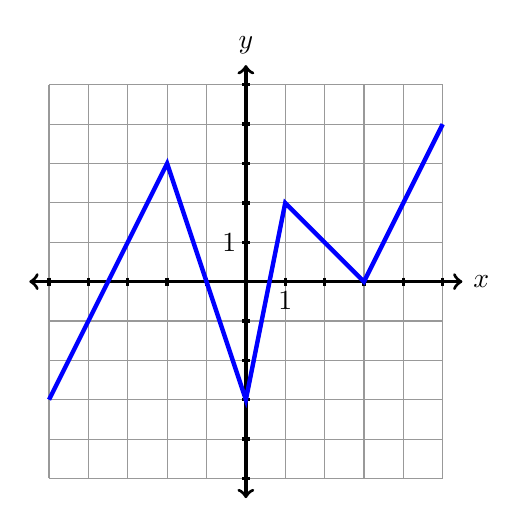
\begin{tikzpicture}[scale=0.5]
\draw [gray!80] (-5,-5) grid (5,5);
\draw[<->, very thick] (-5.5,0) -- (5.5,0) node [right] {$x$};
\draw[<->, very thick] (0,-5.5) -- (0,5.5) node [above] {$y$};
\foreach \x in {-5,-4,...,5}
\draw[very thick] (\x, 0.1) -- (\x, -0.1);
\foreach \y in {-5,-4,...,5}
\draw[very thick] (0.1,\y) -- (-0.1,\y);
\node at (1,0) [below] {$1$};
\node at (0,1) [left] {$1$}; 
\coordinate (A) at (-5,-3);
\coordinate (B) at (-3,1);
\coordinate (C) at (-2,3);
\coordinate (D) at (0,-3);
\coordinate (E) at (1,2);
\coordinate (F) at (3,0);
\coordinate (G) at (5,4);
\draw[color=blue, ultra thick] (A)--(B)--(C)--(D)--(E)--(F)--(G);
\end{tikzpicture}
\end{center}
\begin{multicols}{4}
\begin{enumerate}		\setcounter{enumi}{\value{Review}}
	\item $f(-5)$
	\item $f(-4)$
	\item $f(-1)$
	\item $f(-2)$
\end{enumerate}		\setcounter{Review}{\value{enumi}}
\end{multicols}
\begin{multicols}{4}
\begin{enumerate}		\setcounter{enumi}{\value{Review}}
	\item $f(3)$
	\item $f(4)$
	\item $f(2)$
	\item $f(0)$
\end{enumerate}		\setcounter{Review}{\value{enumi}}
\end{multicols}

\newpage

\section{Answer Key}

\begin{enumerate}
	\item $\frac{49}{5}$
    \item $\frac{39}{5}$
    \item $\frac{48}{5}$
    \item $-3$
    \item $-1$
    \item 0 
    \item 3
    \item 0
    \item 2
    \item 1
    \item $-3$
\end{enumerate}